\documentclass[11pt]{amsart}


%The package below let's us add todos to the document in a way that will stand out at a glance.  It will also list all of the current things to do, with their respective page numbers on the first page of the document.  You can add a todo like this:
%
%		Text text text \todo{change this text to something useful!}
%
%Among other things, you can edit the color of a todo:
%
%		\todo[color=\ltblue]{this todo will have a light blue background!}
%
%And you can include the todo as a line in the text, rather than in the margins:
%
%		\todo[inline]{this will appear in the middle of the page}

\usepackage[colorinlistoftodos, textsize=tiny]{todonotes}
\def\ltblue{blue!20!white}
\def\ltgreen{green!20!white}

\usepackage{amsmath,amssymb,amsthm, MnSymbol}
\usepackage{enumerate}
\usepackage{natbib}

\usepackage{tikz}
\usepackage{tikz-cd}
\usetikzlibrary{matrix, calc, arrows}
\usepackage{latexsym,amscd,epsfig,verbatim}
\usepackage[margin=1in,letterpaper,portrait]{geometry}

\newtheorem{thm}{Theorem}[section]
\newtheorem{lem}[thm]{Lemma}
\newtheorem{prop}[thm]{Proposition}
\newtheorem{cor}[thm]{Corollary}
\newtheorem{conj}[thm]{Conjecture}

%\usepackage[all]{xy}
\theoremstyle{definition}
\newtheorem{defn}[thm]{Definition}
\newtheorem{note}[thm]{Notation}
\newtheorem{rem}[thm]{Remark}
\newcommand\fri{s_4^{-1}}
\newcommand\fr{s_4}
\newcommand\tri{s_3^{-1}}
\newcommand\tr{s_3}
\newcommand\twi{s_2^{-1}}
\newcommand\tw{s_2}
\newcommand\oni{s_1^{-1}}
\newcommand\on{s_1}
\newcommand\V{V(\Gamma)}

\makeatletter
\providecommand\@dotsep{5}
\def\listtodoname{List of Todos}
\def\listoftodos{\@starttoc{tdo}\listtodoname}
\makeatother


\begin{document}
%This adds the list of todos to the first page.
\listoftodos




\title{Artin Group Presentations of Reflection Groups}
\author{Jacob Haley, David Hemminger, Aaron Landesman, Hailee Peck}
\address{you can put addresses for authors\\
here \\
Jacob: 225 St. Edward's Hall; Notre Dame, IN 46556}
\email{..., jhaley3@nd.edu, david.hemminger@duke.edu, hpeck@millikin.edu}
\date{\today}
\keywords{Artin group, cluster algebra, diagram representations}

\begin{abstract}
In 2003, Fomin and Zelevinsky proved that finite-type cluster algebras can be classified by Dynkin diagrams. Then in 2013, Barot and Marsh defined the presentation of a reflection group associated to a Dynkin diagram in terms of an edge-weighted, oriented graph, and proved that this group is invariant (up to isomorphism) under diagram mutations. In this paper, we extend Barot and Marsh's results to Artin group presentations, defining new relations for when the generators are not self-inverses and again showing mutation-invariance for these presentations.
\end{abstract}

\maketitle

\section{Introduction \& Motivation}
\label{sec:Intro}


In \cite{FZ02}, Fomin and Zelevinsky first introduced the concept of cluster algebras. This introductory paper focused on structural features of cluster algebras, specifically that, in a given cluster, when any cluster variable is viewed as a rational function in the variables of the given cluster, this cluster variable is a Laurent polynomial. \todo{The first sentence seems to be run on, and I'm very confused by it} Fomin and Zelevinsky defined cluster algebras in order to make further strides in the areas of representation theory, Lie theory, and total positivity. Since then, the study of cluster algebras has provided a motivation for applications in various other areas of mathematics, including quiver representations. Of particular interest were \textit{finite-type} cluster algebras, that is, cluster algebras whose variables are generated through mutation on a finite number of \textit{seeds}. In the sequel to their introductory paper (\cite{FZ03}), Fomin and Zelevinsky introduce the concept of \textit{mutation equivalence} between diagrams, proving that a connected graph is mutation equivalent to an oriented Dynkin diagram if and only if all mutation equivalent graphs have edge weights not exceeding 3. In particular, this proves that finite-type cluster algebras can be classified by Dynkin diagrams. \\
\indent Barot and Marsh extended Fomin and Zelevinsky's results in \cite{BM13}, providing a presentation of the reflection group associated to a Dynkin diagram with generators that correspond to elements of a companion basis associated to a seed of a finite-type cluster algebra. They also proved that this group presentation is invariant up to isomorphism under the mutation equivalence relation.


\todo{Fix mathscr on Hailee's first theorem which is commented out}

\iffalse
\begin{thm}\cite[Theorem 5.4]{BM13}
\begin{enumerate}
\item Let $\Gamma$ be a diagram of finite type and $\Gamma^{\prime} = \mu_k(\Gamma)$ the mutation of $\Gamma$ at vertex $k$. Then $W_{\Gamma} \cong W_{\Gamma^{\prime}}$.
\item Let $\mathscr{A}$ be a cluster algebra of finite type. Then the groups $W_{\Gamma}$ associated to the diagrams $\Gamma$ arising from the seeds of $\mathscr{A}$ are all isomorphic (to the reflection group associated to the Dynkin diagram associated to $\mathscr{A}$).
\end{enumerate}
\end{thm}
\fi


That is, given a diagram $\Gamma$ and a diagram mutation equivalent to $\Gamma$, denoted $\Gamma^{\prime} = \mu_k(\Gamma)$, they proved that $W_{\Gamma} \cong W_{\Gamma^{\prime}}$, where $W_{\Gamma}$ and $W_{\Gamma^{\prime}}$ are the group representations corresponding to $\Gamma$ and $\Gamma^{\prime}$, respectively. \\

\indent Section \ref{sec:main_definitions} provides the necessary definitions and fundamental results from \cite{BM13} to motivate our own results. For further definitions and references on the topic, we refer the reader to \cite{FZ02}. Section \ref{sec:finite-type_diagrams}  will review theory from \cite{FZ02}, \cite{FZ03} as well as review the classifications (from \cite{BM13}) of mutations of diagrams and their oriented chordless cycles. In Section \ref{sec:defn_artingroup}, we define the appropriate relations for our Artin group presentations. Section \ref{sec:one_relation} specifies how certain relations in chordless cycles imply other relations in those chordless cycles. Finally, Section \todo{for example}\ref{sec:proof_of_main} will provide the proof that the Artin group defined for a diagram $\Gamma$ is invariant up to isomorphism under mutations of $\Gamma$. \\

\section{Definitions and Notation}
\label{sec:main_definitions}

We begin by introducing some preliminary notations and definitions which will aid the reader in understanding the results in the following sections. For further references on cluster algebras, we refer the reader to \cite{FZ02} and \cite{FZ03} and for a more detailed description of Artin group presentations, we direct attention to \cite{FN61}. We also provide references to several lemmas and propositions from \cite{BM13} which were helpful in formulating our own results. \\


A \textit{cluster algebra} is an integral domain which can be generated by a set of elements called \textit{cluster variables} that satisfy certain exchange relations. Following the style of \cite{FZ02} and \cite{BM13}, we will define cluster algebras in terms of \textit{skew-symmetrisable} matrices (that is, a matrix $B$ such that there exists a diagonal matrix $D$ of the same size with $D_{ii} >0$ such that $DB$ is skew-symmetric). Let $\mathbb{F} = \mathbb{Q}(u_1, u_2, \ldots, u_n)$ be the field of rational functions in $n$ indeterminates over $\mathbb{Q}$. We will define an \textit{intial seed} for the cluster algebra to be a fixed pair $(\textbf{x}, B)$, where $\textbf{x} = \{x_1, \ldots, x_n\}$ is a free generating set of $\mathbb{F}$ and $B$ is an $n \times n$ skew-symmetric matrix. Define $x_k^{\prime} \in \mathbb{F}$ by the \textit{exchange relation}
\begin{displaymath}
x_k^{\prime}x_k = \prod_{B_{ik} > 0}{x_i^{B_{ik}}} + \prod_{B_{ik} < 0}{x_i^{-B_{ik}}}
\end{displaymath}
Then, given an initial seed $(\textbf{x}, B)$ and $k \in {1,2,\ldots,n}$, we can define a \textit{mutation} of the seed at $k$, denoted $\mu_k(\boldsymbol{x}, B) = (\textbf{x}^{\prime}, B^{\prime})$ where:
\begin{displaymath}
B_{ij}^{\prime} = \begin{cases} - B_{ij} & \mbox{ if } i = k \mbox{ or } j = k;\\
																B_{ij} + \frac{|B_{ik}|B_{kj} + B_{ik}|B_{kj}|}{2} & \mbox{ otherwise. }\\
									\end{cases}
\end{displaymath}
and $\textbf{x}^{\prime} = {x_1, x_2, \ldots, x_{k-1}, x_k^{\prime}, x_{k+1}, \ldots, x_n}$. 
Such a mutation or a sequence of such mutations generate \textit{seeds} which in turn generate all cluster variables in that, for each $\textbf{x} = {x_1, \ldots, x_n}$ corresponding to a seed of the cluster algebra, the entries $x_i$ are the cluster variables. \\

 A cluster algebra is said to be of \textit{finite type} if the number of cluster variables that generate it is finite (if it has finitely many seeds). For each finite type cluster algebra, we can associate to its corresponding skew-symmetrisable matrix an edge-weighted, oriented graph, called a \textit{diagram}. We will often denote this diagram by $\Gamma$, and the vertex set of $\Gamma$ by $\V$. We will denote two connected vertices by $i \rightarrow j$, or by $i\--\ j$ if the orientation is not specified. The diagram is determined by, for $i, j \in \V$, $i \xrightarrow{w} j$ if and only if $B_{ij} > 0$ and $w = |B_{ij}B_{ji}|$ is the weight of the edge. A skew-symmetrisable matrix $B$ is \textit{2-finite} if $|B_{ij}B_{ji}| \leq 3$ for $i, j \in {1, \ldots, n}$.  By \cite[7.5]{FZ02}, we have that if $B$ is 2-finite, all 3-cycles in the unoriented graph underlying our diagram must be oriented cyclically. \\

Just as we can define mutations of the seeds of a cluster variable, we can also define mutations of a diagram associated to a cluster algebra of finite type by the following set of rules:
\begin{prop}\cite[Proposition 1.4]{BM13}
Let $B$ be a 2-finite skew-symmetrisable matrix. Then $\Gamma(\mu_k(B))$ is uniquely determined by $\Gamma(B)$ as follows: 
\begin{itemize}
\item Reverse the orientations of all edges in $\Gamma(B)$ incident with $k$ (leaving the weights unchanged)
\item For any path in $\Gamma(B)$ of form $i \xrightarrow{a} k \xrightarrow{b} j$ (i.e. with $a,b$ positive), let $c$ be the weight on the edge $j \rightarrow i$, taken to be zero if there is no such arrow. Let $c'$ be determined by $c'\geq 0$ and 
$c+c' =$ max$(a,b)$. 
Then $\Gamma(B)$ changes in a predetermined way, \todo{Say what this way is?} taking the case $c' = 0$ to mean no arrow between $i$ and $j$.
\end{itemize}
\end{prop}

\begin{note}
We notate this mutation of $\Gamma(B)$ at vertex $k$ by $\mu_k(\Gamma)$. \\
\end{note}


\indent Given a diagram $\Gamma$, Barot and Marsh define for $i, j \in \V$,
\begin{displaymath}
m_{ij} = \begin{cases}    2 & \mbox{if } i \mbox{ and } j \mbox{ are not connected;} \\
																	3 & \mbox{if } i \mbox{ and } j \mbox{ are connected by an edge of weight } 1;\\
																	4 & \mbox{if } i \mbox{ and } j \mbox{ are connected by an edge of weight } 2;\\
																	6 & \mbox{if } i \mbox{ and } j \mbox{ are connected by an edge of weight } 3.\\
					\end{cases}
\end{displaymath}	

Then, they define $W(\Gamma)$ to be the group generated by $s_i$, for $i \in \V$, under the following relations. Note that $e$ will denote the identity element of $W(\Gamma)$. 
\begin{enumerate}
\item $s_i^2 = e$ for all $i$;
\item $(s_is_j)^{m_{ij}} = e$ for all $i \neq j$;
\item For any chordless cycle $C$ in $\Gamma$, where
\begin{displaymath}
C = i_0 \rightarrow i_1 \rightarrow \cdots \rightarrow i_{d-1} \rightarrow i_0
\end{displaymath}
and all of the weights $w_k$ are $1$ or $w_0 = 2$, we have
\begin{displaymath}
(s_{i_0}s_{i_1}\cdots s_{i_{d-2}}s_{i_{d-1}}s_{i_{d-2}}\cdots s_{i_1})^2 =e.
\end{displaymath}
\todo{Maybe it's worth presenting definition 2.4 before this, and then saying it is equivalent to removing certain the (R3)(b) relations. Don't they actually present the definition you refer to in Definition 2.4 as the presentation? You say it is an alteration there, but I think it's the original definition}
\end{enumerate}

Using this group presentation, Barot and Marsh state the following result:
\begin{thm}\cite[Theorem A]{BM13}
Let $\Gamma$ be the diagram associated to a seed in a cluster algebra of finite type. Then $W(\Gamma)$ is isomorphic to the corresponding reflection group.
\end{thm}

In Section 3 of \cite{BM13}, Barot and Marsh provide an alteration of the group $W(\Gamma)$ in order to extend the group definition to any diagram of finite type. The group they define is as follows: 

\begin{defn}
Let $W_{\Gamma}$ be the group with generators $s_i, i = 1,2,\ldots, n$, subject to the following relations:
\begin{itemize}
\item{(R1)} $s_i^2 = e$ for all $i$
\item{(R2)} $\left(s_is_j\right)^{m_{ij}} = e$ for all $i \neq j$
\end{itemize}
Furthermore, for a chordless cycle $C : i_0 \rightarrow i_1 \rightarrow \cdots \rightarrow i_{d-1} \rightarrow i_0$ and for $a = 0,1,2,\ldots, d-1$, define \textbf{$r\left(i_a, i_{a+1}\right) = s_{i_a}s_{i_{a+1}} \cdots s_{i_{a+d-1}}s_{i_{a+d-2}} \cdots s_{i_{a+1}}$}.\\

\vspace{0.1cm}
Then we have the following relations:
\begin{itemize}
\item{(R3)(a)} If all the weights in the edges of $C$ are $1$, then $r(i_a, i_{a+1})^2 = e$
\item{(R3)(b)} If $C$ has some edges of weight $2$, then $r(i_a, i_{a+1})^k = e$ where $k = 4-w_a$ and $w_a$ is the weight of the edge $i_a\--\ i_{a-1}$
\end{itemize}
\end{defn}

Defining the group $W_{\Gamma}$ with relations as shown above allows them to prove certain characteristics of the interaction between the relations in this group for the chordless cycles underlying the diagrams in question. In particular, they prove the following result.
\begin{thm}\cite[Theorem 5.4a]{BM13}
Let $\Gamma$ be a diagram of finite type and $\Gamma^{\prime} = \mu_k(\Gamma)$ the mutation of $\Gamma$ at vertex $k$. Then $W_{\Gamma} \cong W_{\Gamma^{\prime}}$.
\end{thm}

The rest of the paper will be devoted to building up analogous relations, defined in ~\ref{grp def} to prove a similar result in the case of Artin groups.


\section{Diagrams of Finite Type}
\label{sec:finite-type_diagrams}

In this section, we shall review the structure of diagrams of finite type, and how their cycles are affected by mutation. This section is simply a recap of \cite[Section 2]{BM13}.

\begin{defn}
A {\it chordless cycle} of an unoriented graph $G$ is a connected subgraph $H \subset G$ such that the number of vertices in $H$ is equal to the number of edges in $H,$ and the edges in $H$ form a single cycle.  
\end{defn}

\begin{prop}
Let $\Gamma$ be a diagram of finite type. Then, a chordless cycle in the unoriented graph of $\Gamma$ is cyclically oriented in $\Gamma$. Furthermore, the unoriented graph underlying the cycle must either be a cycle such that all edges have weight 1, a triangle with two edges of weight 2 and one of weight 1, or a square with two opposite edges of weight 2 and two opposite edges of weight 1, as pictured below.

\begin{tikzpicture}[baseline=-0.5ex]
 \matrix[matrix of math nodes,column sep={40pt,between origins},row
    sep={40pt,between origins},nodes={asymmetrical rectangle}] at (0,0)
  {
    & &|[name = ul]|\circ& |[name = ur]|\circ&\\
    %
    &|[name=lu]| \circ &&&|[name=ru]| \circ \\
     & |[name = ld]|\circ&&& |[name = rd]|\circ\\
    %
    &&|[name=dl]| \circ &|[name=dr]| \circ &\\
  };
\draw
  (ul) -- node[above] {1} (ur)
  ;
  \draw
  (ul) -- node[left]{1}(lu)
  ;
  \draw
  (dr) -- node[right]{1}(rd)
  ;
  \draw
  (lu) -- node[left]{1}(ld)
  ;
  \draw
  (ru) -- node[right]{1}(rd)
  ;
  \draw
  (ur) -- node[right]{1}(ru)
  ;
  \draw
  (dl) -- node[left]{1}(ld)
  ;
  \draw[dotted]
  (dl) -- (dr)
  ; 
 \matrix[matrix of math nodes,column sep={40pt,between origins},row
    sep={40pt,between origins},nodes={asymmetrical rectangle}] at (6,0)
  {
    & |[name = ul]|\circ& |[name = ur]|\circ\\
    %
    &|[name=dl]| \circ &|[name=dr]| \circ \\
  };
\draw
  (ul) -- node[above] {1} (ur)
  ;
  \draw
  (dl) -- node[left]{2}(ul)
  ;
  \draw
  (dr) -- node[below]{1}(dl)
  ;
  \draw
  (ur) -- node[right]{2} (dr)
  ; 
   \matrix[matrix of math nodes,column sep={25pt,between origins},row
    sep={40pt,between origins},nodes={asymmetrical rectangle}] at (10,0)
  {
    && |[name = u]|\circ& \\
    %
    &|[name=dl]| \circ & &|[name=dr]| \circ \\
  };
\draw
  (u) -- node[right] {2} (dr)
  ;
  \draw
  (dl) -- node[left]{2}(u)
  ;
  \draw
  (dr) -- node[below]{1}(dl)
  ;
  
   \end{tikzpicture}

\end{prop}
\begin{proof}
See \cite[Proposition 2.1]{BM13}.
\end{proof}

\begin{cor}
Let $\Gamma$ be the a graph of finite type and suppose there are three vertices, labeled $i,j,k$ with both $i,j$ connected to $k.$ Then mutation at $k$ on the induced subdiagram appear as in one of the following figures, either from left to right or right to left, up to switching $i$ and $j,$

\begin{enumerate}[(a)]
\item 	
	\begin{tikzpicture}[baseline=-0.5ex]
	 \matrix[matrix of math nodes,column sep={25pt,between origins},row
    sep={40pt,between origins},nodes={asymmetrical rectangle}] at (0,0)
  {
    && |[name = u]|\bullet& \\
    %
    &|[name=dl]| \circ & &|[name=dr]| \circ \\
  };
\draw[->]
  (dr) to node[right] {1} (u)
  ;
  \draw[->]
  (dl)to node[left]{1}(u) 
  ;
  \node [yshift = .4 cm] at (u){k};
    \node [yshift = -.4 cm,xshift = .4 cm] at (dr){j};
    \node [yshift = -.4 cm,xshift = -.4 cm] at (dl){i};
    \matrix[matrix of math nodes,column sep={25pt,between origins},row
    sep={40pt,between origins},nodes={asymmetrical rectangle}] at (6,0)
  {
    && |[name = u]|\bullet& \\
    %
    &|[name=dl]| \circ & &|[name=dr]| \circ \\
  };
\draw[->]
   (u)to node[right] {1} (dr)
  ;
  \draw[->]
  (u) to node[left]{1}(dl)
  ;
  \node [yshift = .4 cm] at (u){k};
    \node [yshift = -.4 cm,xshift = .4 cm] at (dr){j};
    \node [yshift = -.4 cm,xshift = -.4 cm] at (dl){i};
   \end{tikzpicture}
	\item 	
	\begin{tikzpicture}[baseline=-0.5ex]
	 \matrix[matrix of math nodes,column sep={25pt,between origins},row
    sep={40pt,between origins},nodes={asymmetrical rectangle}] at (0,0)
  {
    && |[name = u]|\bullet& \\
    %
    &|[name=dl]| \circ & &|[name=dr]| \circ \\
  };
\draw[->]
  (u) to node[right] {1} (dr)
  ;
  \draw[->]
  (dl)to node[left]{1}(u) 
  ;
  \node [yshift = .4 cm] at (u){k};
    \node [yshift = -.4 cm,xshift = .4 cm] at (dr){j};
    \node [yshift = -.4 cm,xshift = -.4 cm] at (dl){i};
    \matrix[matrix of math nodes,column sep={25pt,between origins},row
    sep={40pt,between origins},nodes={asymmetrical rectangle}] at (6,0)
  {
    && |[name = u]|\bullet& \\
    %
    &|[name=dl]| \circ & &|[name=dr]| \circ \\
  };
\draw[->]
  (dr) to node[right] {1}(u) 
  ;
  \draw[->]
  (u) to node[left]{1}(dl)
  ;
  \draw[->]
  (dl) to node[below]{1}(dr)
  ;
  \node [yshift = .4 cm] at (u){k};
    \node [yshift = -.4 cm,xshift = .4 cm] at (dr){j};
    \node [yshift = -.4 cm,xshift = -.4 cm] at (dl){i};
   \end{tikzpicture}

\item 	
	\begin{tikzpicture}[baseline=-0.5ex]
	 \matrix[matrix of math nodes,column sep={25pt,between origins},row
    sep={40pt,between origins},nodes={asymmetrical rectangle}] at (0,0)
  {
    && |[name = u]|\bullet& \\
    %
    &|[name=dl]| \circ & &|[name=dr]| \circ \\
  };
\draw[->]
  (dr) to node[right] {2} (u)
  ;
  \draw[->]
  (dl)to node[left]{1}(u) 
  ;
  \node [yshift = .4 cm] at (u){k};
    \node [yshift = -.4 cm,xshift = .4 cm] at (dr){j};
    \node [yshift = -.4 cm,xshift = -.4 cm] at (dl){i};
    \matrix[matrix of math nodes,column sep={25pt,between origins},row
    sep={40pt,between origins},nodes={asymmetrical rectangle}] at (6,0)
  {
    && |[name = u]|\bullet& \\
    %
    &|[name=dl]| \circ & &|[name=dr]| \circ \\
  };
\draw[->]
   (u)to node[right] {2} (dr)
  ;
  \draw[->]
  (u) to node[left]{1}(dl)
  ;
  \node [yshift = .4 cm] at (u){k};
    \node [yshift = -.4 cm,xshift = .4 cm] at (dr){j};
    \node [yshift = -.4 cm,xshift = -.4 cm] at (dl){i};
   \end{tikzpicture}
   \item 	
	\begin{tikzpicture}[baseline=-0.5ex]
	 \matrix[matrix of math nodes,column sep={25pt,between origins},row
    sep={40pt,between origins},nodes={asymmetrical rectangle}] at (0,0)
  {
    && |[name = u]|\bullet& \\
    %
    &|[name=dl]| \circ & &|[name=dr]| \circ \\
  };
\draw[->]
  (u) to node[right] {1} (dr)
  ;
  \draw[->]
  (dl) to node[left]{2}(u)
  ;
  \node [yshift = .4 cm] at (u){k};
    \node [yshift = -.4 cm,xshift = .4 cm] at (dr){j};
    \node [yshift = -.4 cm,xshift = -.4 cm] at (dl){i};
    \matrix[matrix of math nodes,column sep={25pt,between origins},row
    sep={40pt,between origins},nodes={asymmetrical rectangle}] at (6,0)
  {
    && |[name = u]|\bullet& \\
    %
    &|[name=dl]| \circ & &|[name=dr]| \circ \\
  };
\draw[->]
  (dr)to node[right] {1} (u) 
  ;
  \draw[->]
  (u) to node[left]{2}(dl)
  ;
  \draw[->]
  (dl) to node[below]{2}(dr)
  ;
  \node [yshift = .4 cm] at (u){k};
    \node [yshift = -.4 cm,xshift = .4 cm] at (dr){j};
    \node [yshift = -.4 cm,xshift = -.4 cm] at (dl){i};
   \end{tikzpicture}
   \item 	
	\begin{tikzpicture}[baseline=-0.5ex]
	 \matrix[matrix of math nodes,column sep={25pt,between origins},row
    sep={40pt,between origins},nodes={asymmetrical rectangle}] at (0,0)
  {
    && |[name = u]|\bullet& \\
    %
    &|[name=dl]| \circ & &|[name=dr]| \circ \\
  };
\draw[->]
  (u) to node[right] {2} (dr)
  ;
  \draw[->]
  (dl) to node[left]{1}(u)
  ;
  \node [yshift = .4 cm] at (u){k};
    \node [yshift = -.4 cm,xshift = .4 cm] at (dr){j};
    \node [yshift = -.4 cm,xshift = -.4 cm] at (dl){i};
    \matrix[matrix of math nodes,column sep={25pt,between origins},row
    sep={40pt,between origins},nodes={asymmetrical rectangle}] at (6,0)
  {
    && |[name = u]|\bullet& \\
    %
    &|[name=dl]| \circ & &|[name=dr]| \circ \\
  };
\draw[->]
  (dr) to node[right] {2} (u)
  ;
  \draw[->]
  (u) to node[left]{1}(dl)
  ;
  \draw[->]
  (dl) to node[below]{2}(dr)
  ;
  \node [yshift = .4 cm] at (u){k};
    \node [yshift = -.4 cm,xshift = .4 cm] at (dr){j};
    \node [yshift = -.4 cm,xshift = -.4 cm] at (dl){i};
   \end{tikzpicture}
	\item 	
	\begin{tikzpicture}[baseline=-0.5ex]
	 \matrix[matrix of math nodes,column sep={25pt,between origins},row
    sep={40pt,between origins},nodes={asymmetrical rectangle}] at (0,0)
  {
    && |[name = u]|\bullet& \\
    %
    &|[name=dl]| \circ & &|[name=dr]| \circ \\
  };
\draw[->]
   (u) to node[right] {2}(dr)
  ;
  \draw[->]
  (dl) to node[left]{2}(u)
  ;
  \draw[->]
  (dr) to node[below]{1}(dl)
  ;
  \node [yshift = .4 cm] at (u){k};
    \node [yshift = -.4 cm,xshift = .4 cm] at (dr){j};
    \node [yshift = -.4 cm,xshift = -.4 cm] at (dl){i};
    \matrix[matrix of math nodes,column sep={25pt,between origins},row
    sep={40pt,between origins},nodes={asymmetrical rectangle}] at (6,0)
  {
    && |[name = u]|\bullet& \\
    %
    &|[name=dl]| \circ & &|[name=dr]| \circ \\
  };
\draw[->]
  (dr) to node[right] {2} (u)
  ;
  \draw[->]
  (u) to node[left]{2}(dl)
  ;
  \draw[->]
  (dl) to node[below]{1}(dr)
  ;
  \node [yshift = .4 cm] at (u){k};
    \node [yshift = -.4 cm,xshift = .4 cm] at (dr){j};
    \node [yshift = -.4 cm,xshift = -.4 cm] at (dl){i};
   \end{tikzpicture}
\end{enumerate}

\end{cor}
\begin{proof}
See \cite[Corollary 2.3]{BM13}.
\end{proof}



\begin{lem}\label{lem:chordless_cycles}
Let $\Gamma$ be a diagram of finite type with $\Gamma' = \mu_k(\Gamma)$ the mutation of $\Gamma$ at vertex $k.$ Below, we list induced subdiagrams in $\Gamma$ on the left and the resulting induced subdiagrams in $\Gamma'$ with chordless cycles $C'$ on the right, after mutation at $k.$ We draw the diagrams so that $C'$ always has a clockwise cycle. Furthermore, in case $(i),$ we assume $C'$ has at least three vertices, while in case $(j),$ we assume $C'$ has at least four vertices. Every chordless cycle in $\Gamma'$ is of one of these types.

\begin{enumerate}[(a)]
\item 	
	\begin{tikzpicture}[baseline=-0.5ex]
	 \matrix[matrix of math nodes,column sep={25pt,between origins},row
    sep={40pt,between origins},nodes={asymmetrical rectangle}] at (0,0)
  {
    && |[name = u]|\bullet& \\
    %
    &|[name=dl]| \circ & &|[name=dr]| \circ \\
  };
\draw[->]
  (dr) to node[right] {1} (u)
  ;
  \draw[->]
  (u) to node[left]{1}(dl)
  ;
  \node [yshift = .4 cm] at (u){k=2};
    \node [yshift = -.4 cm,xshift = .4 cm] at (dr){3};
    \node [yshift = -.4 cm,xshift = -.4 cm] at (dl){1};
    \matrix[matrix of math nodes,column sep={25pt,between origins},row
    sep={40pt,between origins},nodes={asymmetrical rectangle}] at (6,0)
  {
    && |[name = u]|\bullet& \\
    %
    &|[name=dl]| \circ & &|[name=dr]| \circ \\
  };
\draw[->]
  (u) to node[right] {1} (dr)
  ;
  \draw[->]
  (dl) to node[left]{1}(u)
  ;
  \draw[->]
  (dr) to node[below]{1}(dl)
  ;
  \node [yshift = .4 cm] at (u){k=2};
    \node [yshift = -.4 cm,xshift = .4 cm] at (dr){3};
    \node [yshift = -.4 cm,xshift = -.4 cm] at (dl){1};
   \end{tikzpicture}
   \item 	
	\begin{tikzpicture}[baseline=-0.5ex]
	 \matrix[matrix of math nodes,column sep={25pt,between origins},row
    sep={40pt,between origins},nodes={asymmetrical rectangle}] at (0,0)
  {
    && |[name = u]|\bullet& \\
    %
    &|[name=dl]| \circ & &|[name=dr]| \circ \\
  };
\draw[->]
  (dr) to node[right] {1} (u)
  ;
  \draw[->]
  (u) to node[left]{2}(dl)
  ;
  \node [yshift = .4 cm] at (u){k=2};
    \node [yshift = -.4 cm,xshift = .4 cm] at (dr){3};
    \node [yshift = -.4 cm,xshift = -.4 cm] at (dl){1};
    \matrix[matrix of math nodes,column sep={25pt,between origins},row
    sep={40pt,between origins},nodes={asymmetrical rectangle}] at (6,0)
  {
    && |[name = u]|\bullet& \\
    %
    &|[name=dl]| \circ & &|[name=dr]| \circ \\
  };
\draw[->]
  (u) to node[right] {1} (dr)
  ;
  \draw[->]
  (dl) to node[left]{2}(u)
  ;
  \draw[->]
  (dr) to node[below]{2}(dl)
  ;
  \node [yshift = .4 cm] at (u){k=2};
    \node [yshift = -.4 cm,xshift = .4 cm] at (dr){3};
    \node [yshift = -.4 cm,xshift = -.4 cm] at (dl){1};
   \end{tikzpicture}
   \item 	
	\begin{tikzpicture}[baseline=-0.5ex]
	 \matrix[matrix of math nodes,column sep={25pt,between origins},row
    sep={40pt,between origins},nodes={asymmetrical rectangle}] at (0,0)
  {
    && |[name = u]|\bullet& \\
    %
    &|[name=dl]| \circ & &|[name=dr]| \circ \\
  };
\draw[->]
  (dr) to node[right] {2} (u)
  ;
  \draw[->]
  (u) to node[left]{1}(dl)
  ;
  \node [yshift = .4 cm] at (u){k=2};
    \node [yshift = -.4 cm,xshift = .4 cm] at (dr){3};
    \node [yshift = -.4 cm,xshift = -.4 cm] at (dl){1};
    \matrix[matrix of math nodes,column sep={25pt,between origins},row
    sep={40pt,between origins},nodes={asymmetrical rectangle}] at (6,0)
  {
    && |[name = u]|\bullet& \\
    %
    &|[name=dl]| \circ & &|[name=dr]| \circ \\
  };
\draw[->]
  (u) to node[right] {2} (dr)
  ;
  \draw[->]
  (dl) to node[left]{1}(u)
  ;
  \draw[->]
  (dr) to node[below]{2}(dl)
  ;
  \node [yshift = .4 cm] at (u){k=2};
    \node [yshift = -.4 cm,xshift = .4 cm] at (dr){3};
    \node [yshift = -.4 cm,xshift = -.4 cm] at (dl){1};
   \end{tikzpicture}
	\item 	
	\begin{tikzpicture}[baseline=-0.5ex]
	 \matrix[matrix of math nodes,column sep={25pt,between origins},row
    sep={40pt,between origins},nodes={asymmetrical rectangle}] at (0,0)
  {
    && |[name = u]|\bullet& \\
    %
    &|[name=dl]| \circ & &|[name=dr]| \circ \\
  };
\draw[->]
  (dr) to node[right] {2} (u)
  ;
  \draw[->]
  (u) to node[left]{2}(dl)
  ;
  \draw[->]
  (dl) to node[below]{1}(dr)
  ;
  \node [yshift = .4 cm] at (u){k=2};
    \node [yshift = -.4 cm,xshift = .4 cm] at (dr){3};
    \node [yshift = -.4 cm,xshift = -.4 cm] at (dl){1};
    \matrix[matrix of math nodes,column sep={25pt,between origins},row
    sep={40pt,between origins},nodes={asymmetrical rectangle}] at (6,0)
  {
    && |[name = u]|\bullet& \\
    %
    &|[name=dl]| \circ & &|[name=dr]| \circ \\
  };
\draw[->]
  (u) to node[right] {2} (dr)
  ;
  \draw[->]
  (dl) to node[left]{2}(u)
  ;
  \draw[->]
  (dr) to node[below]{1}(dl)
  ;
  \node [yshift = .4 cm] at (u){k=2};
    \node [yshift = -.4 cm,xshift = .4 cm] at (dr){3};
    \node [yshift = -.4 cm,xshift = -.4 cm] at (dl){1};
   \end{tikzpicture}
	\item 
\begin{tikzpicture}[baseline=-0.5ex]
\matrix[matrix of math nodes,column sep={40pt,between origins},row
    sep={40pt,between origins},nodes={asymmetrical rectangle}] at (0,0)
  {
    & |[name = ul]|\bullet& |[name = ur]|\circ\\
    %
    &|[name=dl]| \circ &|[name=dr]| \circ \\
  };
\draw[->]
  (ur) to node[above] {1} (ul)
  ;
  \draw[->]
  (ul) to node[left]{2}(dl)
  ;
  \draw[->]
  (dr) to node[below]{1}(dl)
  ;
  \draw[->]
  (ur) to node[right]{2} (dr)
  ;
\draw[->]
  (dl) to node[above]{2} (ur)
  ;
    \node [yshift = .4 cm,xshift = -.4 cm] at (ul){k=1};
   \node  [yshift = .4 cm,xshift = .4 cm] at (ur){2};
    \node [yshift = -.4 cm,xshift = .4 cm] at (dr){3};
    \node [yshift = -.4 cm,xshift = -.4 cm] at (dl){4};
    \matrix[matrix of math nodes,column sep={40pt,between origins},row
    sep={40pt,between origins},nodes={asymmetrical rectangle}] at (6,0)
  {
    & |[name = ul]|\bullet& |[name = ur]|\circ\\
    %
    &|[name=dl]| \circ &|[name=dr]| \circ \\
  };
\draw[->]
  (ul) to node[above] {1} (ur)
  ;
  \draw[->]
  (dl) to node[left]{2}(ul)
  ;
  \draw[->]
  (dr) to node[below]{1}(dl)
  ;
  \draw[->]
  (ur) to node[right]{2} (dr)
  ;
    \node [yshift = .4 cm,xshift = -.4 cm] at (ul){k=1};
   \node  [yshift = .4 cm,xshift = .4 cm] at (ur){2};
    \node [yshift = -.4 cm,xshift = .4 cm] at (dr){3};
    \node [yshift = -.4 cm,xshift = -.4 cm] at (dl){4};
 
   \end{tikzpicture}
   
\item \begin{tikzpicture}[baseline=-0.5ex]
\matrix[matrix of math nodes,column sep={40pt,between origins},row
    sep={40pt,between origins},nodes={asymmetrical rectangle}] at (0,0)
  {
    & |[name = ul]|\circ& |[name = ur]|\bullet\\
    %
    &|[name=dl]| \circ &|[name=dr]| \circ \\
  };
\draw[->]
  (ur) to node[above] {1} (ul)
  ;
  \draw[->]
  (dl) to node[left]{2}(ul)
  ;
  \draw[->]
  (dr) to node[below]{1}(dl)
  ;
  \draw[->]
  (dr) to node[right]{2} (ur)
  ;
\draw[->]
  (ul) to node[above]{2} (dr)
  ;
    \node [yshift = .4 cm,xshift = -.4 cm] at (ul){1};
   \node  [yshift = .4 cm,xshift = .4 cm] at (ur){k=2};
    \node [yshift = -.4 cm,xshift = .4 cm] at (dr){3};
    \node [yshift = -.4 cm,xshift = -.4 cm] at (dl){4};
    \matrix[matrix of math nodes,column sep={40pt,between origins},row
    sep={40pt,between origins},nodes={asymmetrical rectangle}] at (6,0)
  {
    & |[name = ul]|\circ& |[name = ur]|\bullet\\
    %
    &|[name=dl]| \circ &|[name=dr]| \circ \\
  };
\draw[->]
  (ul) to node[above] {1} (ur)
  ;
  \draw[->]
  (dl) to node[left]{2}(ul)
  ;
  \draw[->]
  (dr) to node[below]{1}(dl)
  ;
  \draw[->]
  (ur) to node[right]{2} (dr)
  ;
    \node [yshift = .4 cm,xshift = -.4 cm] at (ul){1};
   \node  [yshift = .4 cm,xshift = .4 cm] at (ur){k=2};
    \node [yshift = -.4 cm,xshift = .4 cm] at (dr){3};
    \node [yshift = -.4 cm,xshift = -.4 cm] at (dl){4};
 
   \end{tikzpicture}

   \item  
   \begin{tikzpicture}[baseline=-0.5ex]

    \matrix[matrix of math nodes,column sep={40pt,between origins},row
    sep={40pt,between origins},nodes={asymmetrical rectangle}] at (0,0)
  {
    & |[name = ul]|\bullet& |[name = ur]|\circ\\
    %
    &|[name=dl]| \circ &|[name=dr]| \circ \\
  };
\draw[->]
  (ul) to node[above] {1} (ur)
  ;
  \draw[->]
  (dl) to node[left]{2}(ul)
  ;
  \draw[->]
  (dr) to node[below]{1}(dl)
  ;
  \draw[->]
  (ur) to node[right]{2} (dr)
  ;
    \node [yshift = .4 cm,xshift = -.4 cm] at (ul){k=1};
   \node  [yshift = .4 cm,xshift = .4 cm] at (ur){2};
    \node [yshift = -.4 cm,xshift = .4 cm] at (dr){3};
    \node [yshift = -.4 cm,xshift = -.4 cm] at (dl){4};
 
   \matrix[matrix of math nodes,column sep={40pt,between origins},row
    sep={40pt,between origins},nodes={asymmetrical rectangle}] at (6,0)
  {
    & |[name = ul]|\bullet& |[name = ur]|\circ\\
    %
    &|[name=dl]| \circ &|[name=dr]| \circ \\
  };
\draw[->]
  (ur) to node[above] {1} (ul)
  ;
  \draw[->]
  (ul) to node[left]{2}(dl)
  ;
  \draw[->]
  (dr) to node[below]{1}(dl)
  ;
  \draw[->]
  (ur) to node[right]{2} (dr)
  ;
\draw[->]
  (dl) to node[above]{2} (ur)
  ;
    \node [yshift = .4 cm,xshift = -.4 cm] at (ul){k=1};
   \node  [yshift = .4 cm,xshift = .4 cm] at (ur){2};
    \node [yshift = -.4 cm,xshift = .4 cm] at (dr){3};
    \node [yshift = -.4 cm,xshift = -.4 cm] at (dl){4};
    \end{tikzpicture}
    
    
   \item  
   \begin{tikzpicture}[baseline=-0.5ex]

    \matrix[matrix of math nodes,column sep={40pt,between origins},row
    sep={40pt,between origins},nodes={asymmetrical rectangle}] at (0,0)
  {
    & |[name = ul]|\circ& |[name = ur]|\bullet\\
    %
    &|[name=dl]| \circ &|[name=dr]| \circ \\
  };
\draw[->]
  (ul) to node[above] {1} (ur)
  ;
  \draw[->]
  (dl) to node[left]{2}(ul)
  ;
  \draw[->]
  (dr) to node[below]{1}(dl)
  ;
  \draw[->]
  (ur) to node[right]{2} (dr)
  ;
    \node [yshift = .4 cm,xshift = -.4 cm] at (ul){k};
   \node  [yshift = .4 cm,xshift = .4 cm] at (ur){k=2};
    \node [yshift = -.4 cm,xshift = .4 cm] at (dr){3};
    \node [yshift = -.4 cm,xshift = -.4 cm] at (dl){4};
 
   \matrix[matrix of math nodes,column sep={40pt,between origins},row
    sep={40pt,between origins},nodes={asymmetrical rectangle}] at (6,0)
  {
    & |[name = ul]|\circ & |[name = ur]|\bullet\\
    %
    &|[name=dl]| \circ &|[name=dr]| \circ \\
  };
\draw[->]
  (ur) to node[above] {1} (ul)
  ;
  \draw[->]
  (dl) to node[left]{2}(ul)
  ;
  \draw[->]
  (dr) to node[below]{1}(dl)
  ;
  \draw[->]
  (dr) to node[right]{2} (ur)
  ;
\draw[->]
  (ul) to node[above]{2} (dr)
  ;
    \node [yshift = .4 cm,xshift = -.4 cm] at (ul){1};
   \node  [yshift = .4 cm,xshift = .4 cm] at (ur){k=2};
    \node [yshift = -.4 cm,xshift = .4 cm] at (dr){3};
    \node [yshift = -.4 cm,xshift = -.4 cm] at (dl){4};
    \end{tikzpicture}
    
   \item
   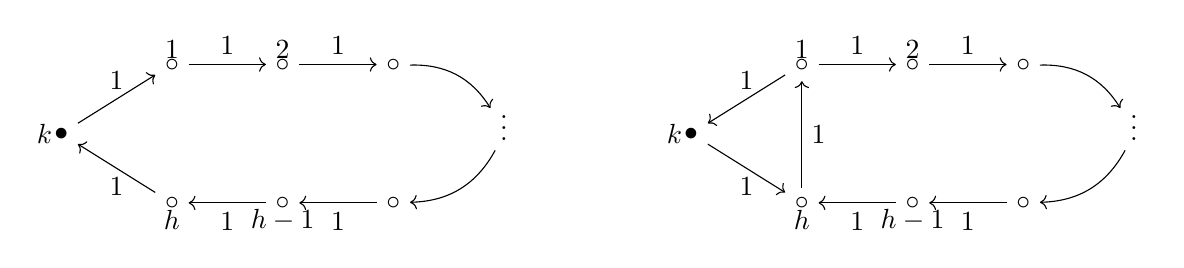
\begin{tikzpicture}[baseline=-0.5ex]
    \matrix[matrix of math nodes,column sep={40pt,between origins},row
    sep={25pt,between origins},nodes={asymmetrical rectangle}] at (0,0)
  {
    & |[name = ul]|\circ& |[name = um]|\circ & |[name = ur]|\circ&\\
    %
    |[name = ml]|\bullet& &&& |[name = mr]|\vdots \\
    %
    & |[name = dl]|\circ& |[name = dm]|\circ & |[name = dr]|\circ&\\
  };
\draw[->]
  (ml) to node[above] {1} (ul)
  ;
  \draw[->]
  (ul) to node[above]{1}(um)
  ;
  \draw[->]
  (um) to node[above]{1}(ur)
  ;
  \draw[->]
  (ur) [bend left] to (mr)
  ;
  \draw[->]
  (mr) [bend left] to (dr)
  ;
  \draw[->]
  (dr) to node[below]{1}(dm)
  ;
  \draw[->]
  (dm) to node[below]{1}(dl)
  ;
  \draw[->]
  (dl) to node[below]{1}(ml)
  ;
    \node at (ml.west){$k$};
    \node at (ul.north){1};
    \node at (um.north){2};
    \node at (dm.south){$h-1$};
    \node at (dl.south){$h$};
    \matrix[matrix of math nodes,column sep={40pt,between origins},row
    sep={25pt,between origins},nodes={asymmetrical rectangle}] at (8,0)
  {
    & |[name = ul]|\circ& |[name = um]|\circ & |[name = ur]|\circ&\\
    %
    |[name = ml]|\bullet& &&& |[name = mr]|\vdots \\
    %
    & |[name = dl]|\circ& |[name = dm]|\circ & |[name = dr]|\circ&\\
  };
\draw[->]
  (ul) to node[above] {1} (ml)
  ;
  \draw[->]
  (ul) to node[above]{1}(um)
  ;
  \draw[->]
  (um) to node[above]{1}(ur)
  ;
  \draw[->]
  (ur) [bend left] to (mr)
  ;
  \draw[->]
  (mr) [bend left] to (dr)
  ;
  \draw[->]
  (dr) to node[below]{1}(dm)
  ;
  \draw[->]
  (dm) to node[below]{1}(dl)
  ;
  \draw[->]
  (ml) to node[below]{1}(dl)
  ;
  \draw[->]
  (dl) to node[right]{1}(ul)
  ;
    \node at (ml.west){$k$};
    \node at (ul.north){1};
    \node at (um.north){2};
    \node at (dm.south){$h-1$};
    \node at (dl.south){$h$};
    \end{tikzpicture}
   
   \item
   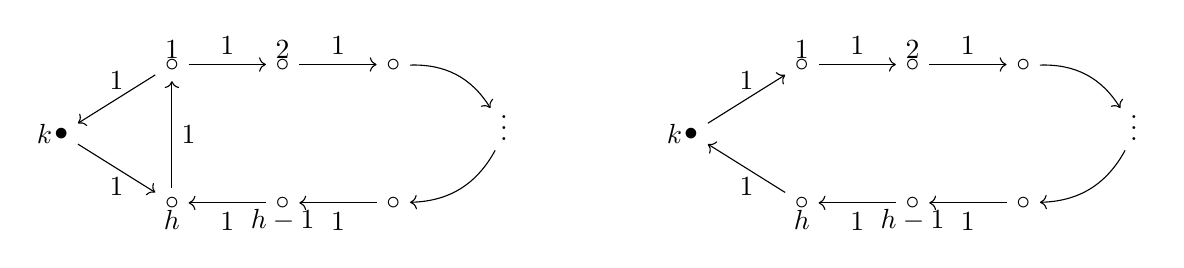
\begin{tikzpicture}[baseline=-0.5ex]
    \matrix[matrix of math nodes,column sep={40pt,between origins},row
    sep={25pt,between origins},nodes={asymmetrical rectangle}] at (8,0)
  {
    & |[name = ul]|\circ& |[name = um]|\circ & |[name = ur]|\circ&\\
    %
    |[name = ml]|\bullet& &&& |[name = mr]|\vdots \\
    %
    & |[name = dl]|\circ& |[name = dm]|\circ & |[name = dr]|\circ&\\
  };
\draw[->]
  (ml) to node[above] {1} (ul)
  ;
  \draw[->]
  (ul) to node[above]{1}(um)
  ;
  \draw[->]
  (um) to node[above]{1}(ur)
  ;
  \draw[->]
  (ur) [bend left] to (mr)
  ;
  \draw[->]
  (mr) [bend left] to (dr)
  ;
  \draw[->]
  (dr) to node[below]{1}(dm)
  ;
  \draw[->]
  (dm) to node[below]{1}(dl)
  ;
  \draw[->]
  (dl) to node[below]{1}(ml)
  ;
    \node at (ml.west){$k$};
    \node at (ul.north){1};
    \node at (um.north){2};
    \node at (dm.south){$h-1$};
    \node at (dl.south){$h$};
    \matrix[matrix of math nodes,column sep={40pt,between origins},row
    sep={25pt,between origins},nodes={asymmetrical rectangle}] at (0,0)
  {
    & |[name = ul]|\circ& |[name = um]|\circ & |[name = ur]|\circ&\\
    %
    |[name = ml]|\bullet& &&& |[name = mr]|\vdots \\
    %
    & |[name = dl]|\circ& |[name = dm]|\circ & |[name = dr]|\circ&\\
  };
\draw[->]
  (ul) to node[above] {1} (ml)
  ;
  \draw[->]
  (ul) to node[above]{1}(um)
  ;
  \draw[->]
  (um) to node[above]{1}(ur)
  ;
  \draw[->]
  (ur) [bend left] to (mr)
  ;
  \draw[->]
  (mr) [bend left] to (dr)
  ;
  \draw[->]
  (dr) to node[below]{1}(dm)
  ;
  \draw[->]
  (dm) to node[below]{1}(dl)
  ;
  \draw[->]
  (ml) to node[below]{1}(dl)
  ;
  \draw[->]
  (dl) to node[right]{1}(ul)
  ;
    \node at (ml.west){$k$};
    \node at (ul.north){1};
    \node at (um.north){2};
    \node at (dm.south){$h-1$};
    \node at (dl.south){$h$};
    \end{tikzpicture}
    
    \item $C$ is an oriented cycle in $\Gamma$ not connected to $k$ and $C'$ is the corresponding cycle in $\Gamma'.$
    
    \item $C$ is an oriented cycle in $\Gamma$ with exactly one vertex in $C$ connected to $k$ by an edge of either weight 1 or 2. Then, $C'$ is the corresponding cycle in $\Gamma'.$  
\end{enumerate}

\end{lem}
\begin{proof}
See \cite[Lemma 2.5]{BM13}.
\end{proof}

\section{The Group of a Diagram in an Artin Group}
\label{sec:defn_artingroup}

\begin{defn} \label{grp def}
For $\Gamma$ a diagram of finite type, we define the associated Artin Group as follows. The associated artin group $W_\Gamma$ is generated by $s_i,$ where there is one $s_i$ for each vertex $i$ in $\Gamma.$ These generators are subject to the relations
\begin{itemize}
	\item[(R2')] For all $i \neq j,$ we add the relations
	\\
$	\begin{cases}
	s_is_j=s_js_i, &\text{ if there is no edge between $i$ and $j$}\\
	s_is_js_i = s_js_is_j &\text{ if there is an edge of weight 1 between $i$ and $j.$}\\
	s_is_js_is_j = s_js_is_js_i &\text{ if there is an edge of weight 2 between $i$ and $j$.}\\
	s_is_js_is_js_is_j = s_js_is_js_is_js_i &\text{ if there is an edge of weight 3 between $i$ and $j$.}
\end{cases}$
\item[(R3')(a)] For every chordless cycle of the form

\begin{tikzcd}
i_0 \arrow{r} & i_1 \arrow{r} & \cdots \arrow{r} & i_{d-1} \arrow{r} & i_0
\end{tikzcd}

such that all edges have weight 1, for all $i,$ with $0 \leq a \leq d-1,$ we include the relation 
\begin{align*}
	s_{a}s_{a+1}^{-1}s_{a+2}^{-1}\dots s_{a-2}^{-1}s_{a-1}s_{a-2}s_{a-3}\dots s_{a+1} = s_{a+1}^{-1}\dots s_{a-3}^{-1}s_{a-2}^{-1}s_{a-1}s_{a-2}\dots s_{a+1}s_{a}.
\end{align*}
Where subscripts are taken $\pmod d.$ 

\item[(R3')(b)] For every chordless cycle of the form \begin{tikzpicture}[baseline=-0.5ex]
    \matrix[matrix of math nodes,column sep={25pt,between origins},row
    sep={40pt,between origins},nodes={asymmetrical rectangle}] at (6,0)
  {
    && |[name = u]|\circ& \\
    %
    &|[name=dl]| \circ & &|[name=dr]| \circ \\
  };
\draw[->]
  (u) to node[right] {1} (dr)
  ;
  \draw[->]
  (dl) to node[left]{2}(u)
  ;
  \draw[->]
  (dr) to node[below]{2}(dl)
  ;
  \node [yshift = .4 cm] at (u){i};
    \node [yshift = -.4 cm,xshift = .4 cm] at (dr){j};
    \node [yshift = -.4 cm,xshift = -.4 cm] at (dl){k};
   \end{tikzpicture}
   we include the three relations
   \begin{enumerate}[(1)]
\item $s_{i}s_{j}^{-1}s_{k}s_{j} = s_{j}^{-1}s_{k}s_{j}s_{i}$
\item $s_{k}s_{i}^{-1}s_{j}s_{i} = s_{i}^{-1}s_{j}s_{i}s_{k}$
\item $s_{j}^{-1}s_{k}^{-1}s_{i}s_{k}s_{j}s_{k}^{-1}s_{i}s_{k}s_{j}^{-1}s_{k}^{-1}s_{i}^{-1}s_{k} = e.$
\end{enumerate}
\item[(R3')(c)] For every chordless cycle of the form
\begin{tikzpicture}[baseline=-0.5ex]
    \matrix[matrix of math nodes,column sep={40pt,between origins},row
    sep={40pt,between origins},nodes={asymmetrical rectangle}] at (6,0)
  {
    & |[name = ul]|\circ & |[name = ur]|\circ\\
    %
    &|[name=dl]| \circ &|[name=dr]| \circ \\
  };
\draw[->]
  (ul) to node[above] {1} (ur)
  ;
  \draw[->]
  (dl) to node[left]{2}(ul)
  ;
  \draw[->]
  (dr) to node[below]{1}(dl)
  ;
  \draw[->]
  (ur) to node[right]{2} (dr)
  ;
    \node [yshift = .4 cm,xshift = -.4 cm] at (ul){i};
   \node  [yshift = .4 cm,xshift = .4 cm] at (ur){j};
    \node [yshift = -.4 cm,xshift = .4 cm] at (dr){k};
    \node [yshift = -.4 cm,xshift = -.4 cm] at (dl){l};
 
   \end{tikzpicture}
   
   we include the two relations
   \begin{enumerate}[(1)]
\item $s_{i}s_{j}^{-1}s_{k}^{-1}s_ls_{k}s_j = s_{j}^{-1}s_{k}^{-1}s_ls_ks_{j}s_{i}$
\item $s_{k}s_{l}^{-1}s_{i}^{-1}s_js_{i}s_l = s_{l}^{-1}s_{i}^{-1}s_js_is_{l}s_{k}$
\end{enumerate}
\end{itemize}
\end{defn}

\begin{rem}
Note that if $\Gamma$ is the graph associated to a Dynkin diagram, then $W_\Gamma$ as we have defined it is precisely the corresponding Artin group corresponding to that Dynkin diagram. This occurs because, in this case, we have no cycles in $\Gamma,$ and so we only have relation of the form $(R2'),$ which define the Artin Group.
\end{rem}

\section{Symmetry among (R3') Relations}
\label{sec:one_relation}

As in \cite{BM13}, given the relations (R2'), many of the relations in (R3')(a) and (b) become redundant. For example,

\begin{lem}
Let $\Gamma$ be a diagram of finite type which contains a chordless cycle C:
\begin{tikzcd}
i_0 \arrow{r} & i_1 \arrow{r} & \cdots \arrow{r} & i_{d-1} \arrow{r} & i_0
\end{tikzcd}
so that all edges have weight 1. Then if W is a group generated by $s_{1}, \dots, s_{n}$ satifying the relations (R2') and $r(i_{a}, i_{a+1})$ for some a $\in \{1, \dots, d\}$, all of the relations in (R3)(a) hold for C.
\end{lem}

\begin{proof}
As in Barot-Marsh, it suffices to prove that the relation r(0, 1) implies the relation r(d-1, 0). So suppose $W_{\gamma}$ satisfies the relation r(0, 1). Then we have 
\begin{align*}
& s_{d-1}s_{0}^{-1}s_{1}^{-1}\dots s_{d-3}^{-1}s_{d-2}s_{d-3}\dots s_1s_0 \\
&= s_{0}^{-1}s_{0}s_{d-1}s_{0}^{-1}s_{1}^{-1}\dots s_{d-3}^{-1}s_{d-2}s_{d-3}\dots s_{1}s_{d-1}^{-1}s_{d-1}s_{0} \\
&= s_{0}^{-1}s_{d-1}^{-1}s_{0}s_{d-1}s_{1}^{-1}\dots s_{d-3}^{-1}s_{d-2}s_{d-3}\dots s_{1}s_{d-1}^{-1}s_{d-1}s_{0} \\
&= s_{0}^{-1}s_{d-1}^{-1}s_{0}s_{1}^{-1}\dots s_{d-3}^{-1}s_{d-1}s_{d-2}s_{d-1}^{-1}s_{d-3}\dots s_{1}s_{d-1}s_{0} \\
&= s_{0}^{-1}s_{d-1}^{-1}(s_{0}s_{1}^{-1}\dots s_{d-3}^{-1}s_{d-2}^{-1}s_{d-1}s_{d-2}s_{d-3}\dots s_{1})s_{d-1}s_{0} \\
&= s_{0}^{-1}s_{d-1}^{-1}(s_{1}^{-1} \dots s_{d-2}^{-1}s_{d-1}s_{d-2}s_{d-3}\dots s_{0})s_{d-1}s_{0} \\
&= s_{0}^{-1}s_{d-1}^{-1}(s_{1}^{-1} \dots s_{d-3}^{-1}s_{d-1}s_{d-2}s_{d-1}^{-1}s_{d-3}\dots s_{0})s_{d-1}s_{0} \\
&= s_{0}^{-1}s_{1}^{-1}\dots s_{d-3}^{-1}s_{d-2}s_{d-3}\dots s_{1}s_{d-1}^{-1}s_{0}s_{d-1}s_{0} \\
&= s_{0}^{-1}s_{1}^{-1}\dots s_{d-3}^{-1}s_{d-2}s_{d-3}\dots s_{1}s_{0}s_{d-1}s_{0}^{-1}s_{0} \\
&= s_{0}^{-1}s_{1}^{-1}\dots s_{d-3}^{-1}s_{d-2}s_{d-3}\dots s_{1}s_{0}s_{d-1} 
\end{align*}
as required. Note that line 3 is equal to 4 and line 7 is equal to line 8 since the cycle is chordless, meaning that $s_{d-1}$ commutes with every element except $s_{0}$ and $s_{d-2}$.
\end{proof}
Furthermore, we obtain similar results for cycles containing edges of weight 2.
\begin{lem} 
Let $\Gamma$ be a diagram of finite type containing a 3-cycle as in (R3')(b) of ~\ref{grp def}. Let W be the group with generators $s_{1}, \dots, s_{n}$ defined by $\Gamma$. Then the relations (1) and (2) of (R3')(b) are equivalent, and they together imply the relation (3).
\end{lem}

\begin{proof}
The equivalence of (1) and (2) follows from the fact that
\begin{align*}
& s_{k}^{-1}s_{j}(s_{i}s_{j}^{-1}s_{k}s_{j}s_{i}^{-1}s_{j}^{-1}s_{k}^{-1}s_{j})s_{j}^{-1}s_{k} \\
&= s_{k}^{-1}s_{j}s_{i}s_{j}^{-1}s_{k}s_{j}s_{i}^{-1}s_{j}^{-1} \\
&= s_{k}^{-1}s_{i}^{-1}s_{j}s_{i}s_{k}s_{i}^{-1}s_{j}^{-1}s_{i}
\end{align*}

In showing that (1) and (2) imply (3), we will underline the terms being manipulated in each line for emphasis.
\begin{align*}
& s_{k}s_{j}s_{k}(s_{j}^{-1}s_{k}^{-1}s_{i}s_{k}s_{j}s_{k}^{-1}s_{i}s_{k}s_{j}^{-1}s_{k}^{-1}s_{i}^{-1}s_{k})s_{k}^{-1}s_{j}^{-1}s_{k}^{-1} \\
&= s_{k}\underline{s_{j}s_{k}s_{j}^{-1}s_{k}^{-1}}s_{i}s_{k}s_{j}s_{k}^{-1}s_{i}s_{k}s_{j}^{-1}s_{k}^{-1}s_{i}^{-1}\underline{s_{k}s_{k}^{-1}}s_{j}^{-1}s_{k}^{-1} \\
&= \underline{s_{k}s_{k}^{-1}}\underline{s_{j}^{-1}s_{k}s_{j}s_{i}}s_{k}s_{j}s_{k}^{-1}s_{i}s_{k}s_{j}^{-1}s_{k}^{-1}s_{i}^{-1}s_{j}^{-1}s_{k}^{-1} \\
&= s_{i}\underline{s_{j}^{-1}s_{k}s_{j}s_{k}}s_{j}s_{k}^{-1}s_{i}s_{k}s_{j}^{-1}s_{k}^{-1}s_{i}^{-1}s_{j}^{-1}s_{k}^{-1} \\
&= s_{i}s_{k}s_{j}\underline{s_{k}s_{j}^{-1}s_{j}s_{k}^{-1}}s_{i}s_{k}s_{j}^{-1}s_{k}^{-1}s_{i}^{-1}s_{j}^{-1}s_{k}^{-1} \\
&= s_{i}\underline{e}s_{k}s_{j}s_{i}s_{k}s_{j}^{-1}s_{k}^{-1}s_{i}^{-1}s_{j}^{-1}s_{k}^{-1} \\
&= s_{i}s_{j}\underline{s_{j}^{-1}s_{k}s_{j}s_{i}}s_{k}s_{j}^{-1}s_{k}^{-1}s_{i}^{-1}s_{j}^{-1}s_{k}^{-1} \\
&= \underline{s_{i}s_{j}s_{i}}s_{j}^{-1}s_{k}s_{j}s_{k}s_{j}^{-1}s_{k}^{-1}s_{i}^{-1}s_{j}^{-1}s_{k}^{-1} \\
&= s_{j}s_{i}\underline{s_{j}s_{j}^{-1}}s_{k}\underline{s_{j}s_{k}s_{j}^{-1}s_{k}^{-1}}s_{i}^{-1}s_{j}^{-1}s_{k}^{-1} \\
&= s_{j}s_{i}\underline{s_{k}s_{k}^{-1}}\underline{s_{j}^{-1}s_{k}s_{j}s_{i}^{-1}}s_{j}^{-1}s_{k}^{-1} \\
&= s_{j}\underline{s_{i}s_{i}^{-1}}s_{j}^{-1}s_{k}\underline{s_{j}s_{j}^{-1}}s_{k}^{-1} \\
&= \underline{s_{j}s_{j}^{-1}}\underline{s_{k}s_{k}^{-1}} \\
&= e
\end{align*}
\end{proof}

\begin{lem} 
Let $\Gamma$ be a diagram of finite type containing a 4-cycle as in (R3')(c) of ~\ref{grp def}. Let W be the group with generators $s_{1}, \dots, s_{n}$ defined by $\Gamma$. Then the relations (1) and (2) of (R3')(c) are equivalent.
\end{lem}

\begin{proof}
We have that
\begin{align*}
& s_{k}^{-1}s_{l}^{-1}s_{j}(s_{i}s_{j}^{-1}s_{k}^{-1}s_{l}s_{k}s_{j}s_{i}^{-1}s_{j}^{-1}s_{k}^{-1}s_{l}^{-1}s_{k}s_{j})s_{j}^{-1}s_{l}s_{k} \\
&= s_{k}^{-1}s_{l}^{-1}(s_{j}s_{i}s_{j}^{-1})(s_{k}^{-1}s_{l}s_{k})(s_{j}s_{i}^{-1}s_{j}^{-1})s_{k}^{-1}s_{l}^{-1}s_{k}s_{l}s_{k} \\
&= s_{k}^{-1}s_{l}^{-1}s_{i}^{-1}s_{j}s_{i}s_{l}s_{k}s_{l}^{-1}s_{i}^{-1}s_{j}^{-1}s_{i}s_{k}^{-1}(s_{l}^{-1}s_{k}s_{l})s_{k} \\
&= s_{k}^{-1}s_{l}^{-1}s_{i}^{-1}s_{j}s_{i}s_{l}s_{k}s_{l}^{-1}s_{i}^{-1}s_{j}^{-1}s_{i}s_{l}
\end{align*}
\end{proof}

Finally, we conclude the section by establishing a relationship between the groups defined by $\Gamma$ and $\Gamma^{op}$, the diagram obtained by reversing all arrows in $\Gamma$.

\begin{lem}\label{lem:op_homomorphism}
Let W$_{\Gamma}$ be generated by $s_{1}, \dots, s_{n}$. Then $s_{1}^{-1}, \dots, s_{n}^{-1}$ satisfy the relations (R2') and (R3') in W$_{\Gamma^{op}}$.
\end{lem}
\begin{proof}
One can see that the inverse elements satisfy (R2') in W$_{\Gamma^{op}}$ by taking the inverse of both sides of the corresponding relation in W$_{\Gamma}$. To see that the elements satisfy (R3') in W$_{\Gamma^{op}}$, note that for a chordless cycle in $\Gamma$ with all weights equal to one, we have $$s_{0}^{-1}\dots s_{d-2}^{-1}s_{d-1}s_{d-2}\dots s_{0} = s_{1}^{-1}\dots s_{d-2}^{-1}s_{d-1}s_{d-2}\dots s_{1}$$ by the relation r(0,1) in (R3') in W$_{\Gamma}$. But then applying relations from (R2'), we have that $$s_{0}^{-1}\dots s_{d-1}s_{d-2}s_{d-1}^{-1}\dots s_{0} = s_{1}^{-1}\dots s_{d-1}s_{d-2}s_{d-1}^{-1}\dots s_{1},$$ and since the cycle in chordless, we then have $$s_{0}^{-1}s_{d-1}\dots s_{d-3}^{-1}s_{d-2}s_{d-3}\dots s_{d-1}^{-1}s_{0} = s_{d-1}s_{1}^{-1}\dots s_{d-3}^{-1}s_{d-2}s_{d-3}\dots s_{1}s_{d-1}^{-1}.$$ Repeating this process, we find that $$s_{0}^{-1}s_{d-1}s_{d-2}\dots s_{2}s_{1}s_{2}^{-1}\dots s_{d-2}^{-1}s_{d-1}^{-1}s_{0} = s_{d-1}s_{d-2}\dots s_{2}s_{1}s_{2}^{-1}\dots s_{d-2}^{-1}s_{d-1}^{-1}.$$ But this occurs if and only if $s_{1}^{-1}, \dots, s_{n}^{-1}$ satisfies the relation r'(0, d-1) in W$_{\Gamma^{op}}.$ 

For a triangle as in (R3')(b) of ~\ref{grp def}, by the relation r'(k, i) we have $$s_{k}s_{i}^{-1}s_{j}s_{i}s_{k}^{-1} = s_{i}^{-1}s_{j}s_{i}.$$ Hence $$s_{k}s_{j}s_{i}s_{j}^{-1}s_{k}^{-1} = s_{j}s_{i}s_{j}^{-1}.$$ But as before, this can occur if and only if $s_{i}^{-1}, s_{j}^{-1}, s_{k}^{-1}$ satisfy the relation r'(k, j) in W$_{\Gamma^{op}}$.

Finally, given a square labeled as in (R3')(c) and the relations r'(1, 2) and r'(3, 4), we have 
\begin{align*}
& s_{j}s_{i}s_{l}s_{k}s_{l}^{-1}s_{i}^{-1} \\
&= s_{i}s_{i}^{-1}s_{j}s_{i}s_{l}s_{k}s_{l}^{-1}s_{i}^{-1} \\
&= s_{i}s_{j}s_{i}s_{j}^{-1}s_{k}^{-1}s_{l}s_{k}s_{i}^{-1} \\
&= s_{i}s_{j}(s_{i}s_{j}^{-1}s_{k}^{-1}s_{l}s_{k}s_{j})s_{j}^{-1}s_{i}^{-1} \\
&= s_{i}s_{j}s_{j}^{-1}(s_{k}^{-1}s_{l}s_{k})s_{j}(s_{i}s_{j}^{-1}s_{i}^{-1}) \\
&= s_{i}s_{l}s_{k}s_{l}^{-1}s_{j}s_{j}^{-1}s_{i}^{-1}s_{j} \\
&= s_{i}s_{l}s_{k}s_{l}^{-1}s_{i}^{-1}s_{j}
\end{align*}
But this relation holds if and only if $s_{i}^{-1}, \dots, s_{l}^{-1}$ satisfy r'(j, i) in W$_{\Gamma^{op}}$. Therefore, we are done.
\end{proof}

\section{Proof of Main Result}\label{sec:proof_of_main}


In this section we prove our main result:


\begin{thm}\label{thm:main}
Let $\Gamma$ be a diagram of finite type, and let $\Gamma^{\prime} = \mu_k(\Gamma)$ be the mutation of $\Gamma$ at vertex $k$.  Then $A_{\Gamma} \cong A_{\Gamma^{\prime}}$\todo{we should pick notation for this}.
\end{thm}

Throughout this section we will fix a diagram of finite type $\Gamma$, a vertex $k$ of $\Gamma$, and write $\Gamma^{\prime} = \mu_k(\Gamma)$.  To help us define an isomorphism from $A_{\Gamma}$ to $A_{\Gamma^{\prime}}$ we define an element $t_i\in A_{\Gamma}$ for each vertex $i\in \Gamma$ by

\begin{displaymath}
t_i = \begin{cases}    s_ks_is_k^{-1} & \mbox{if there is a (possibly weighted) arrow} i \rightarrow k \mbox{ in } \Gamma\\
				s_i & \mbox{otherwise}\\
	\end{cases}
\end{displaymath}

In the proof of Theorem \ref{thm:main} we will use Lemma \ref{lem:op_homomorphism} along with the following proposition, whose proof we will defer until after the proof of Theorem \ref{thm:main}.

\begin{prop}\label{prop:ti_relations}
The elements $t_i$, for $i$ a vertex of $\Gamma$, satisfy the relations $(R2)^{\prime}$ and $(R3)^{\prime}$ associated to $\Gamma^{\prime}$.
\end{prop}


\begin{proof}[Proof of Theorem \ref{thm:main}]
Define a homomorphism $\varphi\colon A(\Gamma^{\prime}) \rightarrow A(\Gamma)$ by sending each generator $s_i\in A(\Gamma^{\prime})$ to $t_i\in A(\Gamma)$.  This gives a well-defined homomorphism by Proposition \ref{prop:ti_relations}.  By Lemma \ref{lem:op_homomorphism}, the homormorphism $\Delta\colon A(\Gamma) \rightarrow A(\Gamma^{op})$ that sends $s_i\in A(\Gamma)$ to $s_i^{-1}$ in $A(\Gamma^{op})$ is well-defined.  Define a homomorphism 
$$\psi = \Delta\circ\varphi\circ\Delta\colon A(\Gamma)\rightarrow A(\Gamma^{op})\rightarrow A(\left(\Gamma^{op}\right)^{\prime}) \rightarrow A(\Gamma^{\prime})$$

Note that here we use the facts that $\left(\Gamma^{op}\right)^{op} = \Gamma$ and $\left(\Gamma^{op}\right)^{\prime} = \left(\Gamma^{\prime}\right)^{op}$.  Suppose that there is an arrow $i\rightarrow k$ in $\Gamma$.  Then there will be an arrow $k\rightarrow i$ in $\Gamma^{op}$ and hence an arrow $i\rightarrow k$ in $\left(\Gamma^{op}\right)^{\prime}$, so we have that

$$\psi\circ\varphi(s_i) = \Delta(\varphi(\Delta(\varphi(s_i)))) = \Delta(\varphi(\Delta(s_ks_is_k^{-1}))) = \Delta(\varphi(s_k^{-1}s_i^{-1}s_k)) = \Delta(s_i^{-1}) = s_i$$

Similarly if there is an arrow $k\rightarrow i$ or no arrow between $i$ and $k$ in $\Gamma$ then there will be an arrow $k\rightarrow i$ or no arrow between $i$ and $k$ in $\left(\Gamma^{op}\right)^{\prime}$, respectively.  In each of these cases we have that

$$\psi\circ\varphi(s_i) = \Delta(\varphi(\Delta(\varphi(s_i)))) = \Delta(\varphi(\Delta(s_i))) = \Delta(\varphi(s_i^{-1})) = \Delta(s_i^{-1}) = s_i$$

Thus $\psi\circ\varphi$ is the identity map on $A(\Gamma^{\prime})$.  By a similar argument $\varphi\circ\psi$ is the identity map on $A(\Gamma)$, and hence $A(\Gamma)\cong A(\Gamma^{\prime}))$.
\end{proof}













\begin{proof}[Proof of Proposition \ref{prop:ti_relations}]
First we check the $(R2)'$ relation for $t_i$ and $t_j$ in the case when $i=k$ or $j=k$.  Without loss of generality suppose that $i=k$.  Note that $m_{ij}^\prime = m_{ij}$.  The only nontrivial case is when there is an arrow $j\rightarrow k =i$.  Since $i$ and $j$ are connected in this case, $m_{ij}$ is one of 3,4, or 6.  Suppose $m_{ij} = 3$.  Then $s_js_is_j = s_is_js_i$, so $s_is_j = s_js_is_js_i^{-1}$, and we have

$$t_it_jt_i = s_is_is_js_i^{-1}s_i = s_is_is_j = s_is_js_is_js_i^{-1} = t_jt_it_j$$

\noindent If $m_{ij} = 4$, then $s_is_js_is_j = s_js_is_js_i$, so $s_is_is_js_is_js_i^{-1} = s_is_js_is_j$ and therefore

$$t_it_jt_it_j = s_is_is_js_i^{-1}s_is_is_js_i^{-1} = s_is_js_i^{1-}s_is_is_js_i^{-1}s_i = t_jt_it_jt_i$$

\noindent If $m_{ij} = 6$, then $s_is_is_js_is_js_is_js_i^{-1} = s_is_js_is_js_is_j$, so 

$$t_it_jt_it_jt_it_j = s_is_is_js_i^{-1}s_is_is_js_i^{-1}s_is_is_js_i^{-1} = s_is_js_i^{-1}s_is_is_js_i^{-1}s_is_is_js_i^{-1}s_i = t_jt_it_jt_it_jt_i$$

Next we check the $(R2)'$ relation for $t_i$ and $t_j$ in the case when at most one of $i$ and $j$ is connected to $k$.  The only nontrivial case is when there is an arrow $i\rightarrow k$ or $j\rightarrow k$.  Without loss of generality, suppose there is an arrow $i\rightarrow k$.  Since $j$ is not connected to $k$, we know that $s_js_k = s_ks_j$.  Suppose $m_{ij} = 2$.  Then $s_is_j = s_js_i$, so we have that

$$t_it_j = s_ks_is_k^{-1}s_j = s_js_ks_is_k^{-1} = t_jt_i$$

\noindent If $m_{ij} = 3$, then $s_is_js_i = s_js_is_j$, so we have that 

$$t_it_jt_i = s_ks_is_k^{-1}s_js_ks_is_k^{-1} = s_ks_is_js_is_k^{-1} = s_ks_js_is_js_k^{-1} = s_js_ks_is_k^{-1}s_j = t_jt_it_j$$

\noindent If $m_{ij} = 4$, then $s_is_js_is_j = s_js_is_js_i$, so we have that

$$t_it_jt_it_j = s_ks_is_k^{-1}s_js_ks_is_k^{-1}s_j = s_ks_is_js_is_js_k^{-1} = s_ks_js_is_js_is_k^{-1} = s_js_ks_is_k^{-1}s_js_ks_is_k^{-1} = s_js_is_js_i$$

\noindent Finally if $m_{ij} = 6$, then $s_is_js_is_js_is_j = s_js_is_js_is_js_i$, so we have that

$$t_it_jt_it_jt_it_j = s_ks_is_k^{-1}s_js_ks_is_k^{-1}s_js_ks_is_k^{-1}s_j = s_ks_is_js_is_js_is_js_k^{-1} = s_ks_js_is_js_is_js_is_k^{-1} = t_jt_it_jt_it_jt_i$$




The remaining $(R2)'$ relations that need to be check are the relations for $t_i$ and $t_j$ when both $i$ and $j$ are connected to $k$.  The possibilities for the subdiagram induced by $i$, $j$, and $k$ are enumerated in \todo{where are they enumerated?}.  We show that $t_i$ and $t_j$ satisfy the $(R2^\prime)$ relations by checking each case.  We also check that the corresponding $(R3^\prime)$ relations hold in cases (b), (d), (e), and (f).


\begin{enumerate}[a)]
\item
\begin{enumerate}[i)]
\item $$t_it_j = s_ks_is_k^{-1}s_ks_js_k^{-1} = s_ks_is_js_k^{-1} = s_ks_js_is_k^{-1} = t_jt_i$$
\item $$t_it_j = s_is_j = s_js_i = t_jt_i$$
\end{enumerate}
\item
\begin{enumerate}[i)]
\item
\begin{align*}
t_it_jt_i &= s_ks_is_k^{-1}s_js_ks_is_k^{-1}\\
&= s_ks_is_js_ks_j^{-1}s_is_k^{-1}\\
&= s_ks_js_is_ks_is_j^{-1}s_k^{-1}\\
&= s_ks_js_ks_is_ks_j^{-1}s_k^{-1}\\
&= s_js_ks_js_is_j^{-1}s_k^{-1}s_j\\
&= s_js_ks_is_k^{-1}s_j\\
&= t_it_jt_i
\end{align*}

\begin{align*}
t_jt_k^{-1}t_it_k &= s_js_k^{-1}s_ks_is_k^{-1}s_k\\
&= s_js_i\\
&= s_is_j\\
&= t_k^{-1}t_it_kt_j\\
\end{align*}

\item $$t_it_j = s_is_ks_js_k^{-1} = s_is_j^{-1}s_ks_j = s_j^{-1}s_ks_js_i = s_ks_js_k^{-1}s_i = t_jt_i$$
\end{enumerate}
\item
\begin{enumerate}[i)]
\item $$t_it_j = s_ks_is_k^{-1}s_ks_js_k^{-1} = s_ks_is_js_k^{-1} = s_ks_js_is_k^{-1} = t_jt_i$$
\item $$t_it_j = s_is_j = s_js_i = t_jt_i$$
\end{enumerate}
\item
\begin{enumerate}[i)]
\item
\begin{align*}
t_it_jt_it_jt_i^{-1}t_j^{-1}t_i^{-1}t_j^{-1} &= s_ks_is_k^{-1}s_js_ks_is_k^{-1}s_js_ks_i^{-1}s_k^{-1}s_j^{-1}s_ks_i^{-1}s_k^{-1}s_j^{-1}\\
&=s_ks_is_k^{-1}s_js_ks_is_js_ks_j^{-1}s_i^{-1}s_js_k^{-1}s_j^{-1}s_i^{-1}s_k^{-1}s_j^{-1}\\
&=s_ks_is_k^{-1}s_ks_js_ks_is_ks_i^{-1}s_k^{-1}s_j^{-1}s_i^{-1}s_k^{-1}s_j^{-1}\\
&=s_ks_js_is_ks_is_ks_i^{-1}s_k^{-1}s_i^{-1}s_k^{-1}s_j^{-1}s_k^{-1}\\
&= e
\end{align*}

We also have
$$t_jt_k^{-1}t_it_k = s_js_k^{-1}s_ks_is_k^{-1}s_k = s_is_j = t_k^{-1}t_it_kt_j$$ 

\item
\begin{align*}
t_it_j &= s_is_ks_js_k^{-1}\\
&= s_is_j^{-1}s_ks_j\\
&= s_j^{-1}s_ks_js_i\\
&= s_ks_js_k^{-1}s_i\\
&= t_jt_i
\end{align*}
\end{enumerate}
\item
\begin{enumerate}[i)]
\item
\begin{align*}
t_it_jt_it_jt_i^{-1}t_j^{-1}t_i^{-1}t_j^{-1} &= s_ks_is_k^{-1}s_js_ks_is_k^{-1}s_js_ks_i^{-1}s_k^{-1}s_j^{-1}s_ks_i^{-1}s_k^{-1}s_j^{-1}\\
&= s_i^{-1}s_ks_is_js_i^{-1}s_ks_is_js_i^{-1}s_k^{-1}s_is_j^{-1}s_i^{-1}s_k^{-1}s_is_j^{-1}\\
&= s_i^{-1}s_ks_js_ks_js_k^{-1}s_j^{-1}s_k^{-1}s_j^{-1}s_i\\
&= e
\end{align*}
We also have
$$ t_jt_k^{-1}t_it_k = s_js_k^{-1}s_ks_is_k^{-1}s_k = s_js_i = s_is_j = t_it_j$$

\item
\begin{align*}
s_k^{-1}t_it_jt_i^{-1}t_j^{-1}s_k &= s_k^{-1}s_is_ks_js_k^{-1}s_i^{-1}s_ks_j^{-1}\\
&= s_is_ks_i^{-1}s_js_is_k^{-1}s_i^{-1}s_j^{-1}\\
&= e
\end{align*}

\end{enumerate}
\item
\begin{enumerate}[i)]
\item
\begin{align*}
s_k^{-1}t_it_jt_it_j^{-1}t_i^{-1}t_j^{-1} &= s_is_k^{-1}s_js_ks_is_k^{-1}s_j^{-1}s_ks_i^{-1}s_k^{-1}s_j^{-1}s_k\\
&= e
\end{align*}

\begin{align*}
t_it_j^{-1}t_kt_jt_i^{-1}t_j^{-1}s_k^{-1}t_j &= s_ks_is_k^{-1}s_j^{-1}s_ks_js_ks_i^{-1}s_k^{-1}s_j^{-1}s_k^{-1}s_j\\
&= s_ks_is_js_ks_j^{-1}s_k^{-1}s_ks_i^{-1}s_k^{-1}s_j^{-1}s_k^{-1}s_j\\
&= s_ks_is_js_ks_j^{-1}s_i^{-1}s_k^{-1}s_j^{-1}s_k^{-1}s_j\\
&= s_ks_is_js_ks_j^{-1}s_i^{-1}s_js_k^{-1}s_j^{-1}s_k^{-1}\\
&= s_ks_js_ks_j^{-1}s_is_i^{-1}s_js_k^{-1}s_j^{-1}s_k\\
&= e\\
\end{align*}

\item This follows from part (i) by symmetry
\end{enumerate}
\end{enumerate}

Next we check that the $t_i$ satisfy the (R3) relations defined by the chordless cycles in $\Gamma'$.  We know that every chordless cycle in $\Gamma'$ arises from a subdiagram of $\Gamma$ in the form of one of the cases of Lemma \ref{lem:chordless_cycles}, so we simply need to check that the corresponding cycle relations hold in each case.  By Lemmas \todo{add relevant lemma references}, we will only need one relation for each cycle, as this relation holding will imply that the others hold as well.  Note that we have already checked cases (a)-(d) above, so we only need to check cases (e)-(l).

\begin{enumerate}[a)]
\setcounter{enumi}{4}
\item
Without loss of generality we label the vertices as follows:\todo{insert diagrams}

\begin{align*}
t_1t_2^{-1}t_3^{-1}t_4t_3t_2 &= (s_1s_2^{-1}s_1^{-1}s_1s_2s_1^{-1})s_1s_1s_2^{-1}s_1^{-1}s_3^{-1}s_4s_3s_1s_2s_1^{-1}\\
&= s_1s_2^{-1}s_1^{-1}\underline{s_1s_2s_1s_2^{-1}s_1^{-1}}s_3^{-1}s_4s_3s_1s_2s_1^{-1}\\
&= s_1s_2^{-1}s_1^{-1}\underline{s_2s_3^{-1}s_4s_3}s_1s_2s_1^{-1}\\
&= s_1s_2^{-1}s_1^{-1}s_3^{-1}s_4s_3\underline{s_2s_1s_2s_1^{-1}}\\
&= s_1s_2^{-1}s_1^{-1}s_3^{-1}s_4s_3s_1s_2s_1^{-1}s_1\\
&= t_2^{-1}t_3^{-1}t_4t_3t_2t_1\\
\end{align*}

\item
\begin{align*}
t_4^{-1}t_1^{-1}t_2^{-1}t_3t_2t_1 &= s_4\underline{s_1^{-1}s_1}s_2^{-1}\underline{s_1^{-1}s_3s_1}s_2 \underline{s_1^{-1}s_1}\\
&= s_4s_2^{-1}s_3s_2\\
&= s_2^{-1}s_3s_2s_4\\
&= (s_1^{-1}s_1)s_2^{-1}(s_1^{-1}\underline{s_1)s_3(s_1^{-1}}s_1)s_2(s_1^{-1}s_1s_4\\
&= s_1^{-1}1s_2^{-1}s_1^{-1}s_3s_1s_2s_1^{-1}s_1s_4\\
&= t_1^{-1}t_1^{-1}t_3t_2t_1t_4\\
\end{align*}

\item
\begin{align*}
t_3t_4^{-1}t_2t_4t_3^{-1}t_4^{-1}t_2^{-1}t_4 &= \underline{s_3s_1}s_4^{-1}s_1^{-1}s_2s_1s_4\underline{s_1^{-1}s_3^{-1}s_1}s_4^{-1}s_1^{-1}s_2^{-1}s_1s_4s_1^{-1}\\
&= s_1\underline{s_3s_4^{-1}s_1^{-1}s_2s_1s_4s_3^{-1}s_4^{-1}s_1^{-1}s_2^{-1}s_1s_4}s_1^{-1}\\
&= s_1s_1^{-1}\\
&= e\\
\end{align*}

\item
\begin{align*}
t_2t_3^{-1}t_4t_3 &= s_2s_3^{-1}\underline{s_1s_4s_1^{-1}}s_3\\
&= s_2s_3^{-1}s_4^{-1}s_1s_4s_3\\
&= s_3^{-1}\underline{s_4^{-1}s_1s_4}s_3s_2\\
&= s_3^{-1}s_1s_4s_1^{-1}s_3s_2\\
&= t_3^{-1}t_4t_3t_2\\
\end{align*}

\item
\begin{align*}
t_1t_2^{-1}t_3^{-1}\cdots t_{h-1}^{-1}t_ht_{h-1}\cdots t_2t_1^{-1}t_2^{-1}\cdots t_{h-1}^{-1}t_h^{-1}t_{h-1}\cdots t_2 &= s_1s_2^{-1}s_3^{-1}\cdots s_{h-1}^{-1}\underline{s_ks_hs_k^{-1}}s_{h-1}\cdots s_2s_1^{-1}s_2^{-1}\cdots s_{h-1}^{-1}\underline{s_ks_h^{-1}s_k^{-1}}s_{h-1}\cdots s_2\\
&= s_1s_2^{-1}s_3^{-1}\cdots s_{h-1}^{-1}s_h^{-1}s_ks_hs_{h-1}\cdots s_2s_1^{-1}s_2^{-1}\cdots s_{h-1}^{-1}s_h^{-1}s_k^{-1}s_hs_{h-1}\cdots s_2\\
&= e\\
\end{align*}

\item
\begin{align*}
& t_ht_k^{-1}t_1^{-1}t_2^{-1}\cdots t_{h-2}^{-1}t_{h-1}t_{h-2}\cdots t_1t_kt_h^{-1}t_k^{-1}t_1^{-1}t_2^{-1}\cdots t_{h-2}^{-1}t_{h-1}^{-1}t_{h-2}\cdots t_2t_1t_k\\
&= s_h\underline{s_k^{-1}s_k}s_1^{-1}\underline{s_k^{-1}}s_2^{-1}\cdots s_{h-2}^{-1}s_{h-1}s_{h-2}\cdots \underline{s_k}s_1\underline{s_k^{-1}s_k}s_h^{-1}\underline{s_k^{-1}s_k}s_1^{-1}\underline{s_k^{-1}}s_2^{-1}\cdots s_{h-2}^{-1}s_{h-1}^{-1}s_{h-2}\cdots s_2 \underline{s_k}s_1\underline{s_k^{-1}s_k}\\
&= s_hs_1^{-1}s_2^{-1}\cdots s_{h-2}^{-1}s_{h-1}s_{h-2}\cdots s_2s_1s_h^{-1}s_1^{-1}s_2^{-1}\cdots s_{h-2}^{-1}s_{h-1}^{-1}s_{h-2}\cdots s_2s_1\\
&= e\\
\end{align*}


\end{enumerate}
\end{proof}



\bibliography{References}
\bibliographystyle{alpha}


\end{document}